%%
%% Capítulo 2: Regras gerais de estilo
%%

\mychapter{Teoria}
\label{Cap:Teoria}


\section{Sistema de controle de acesso}
\label{Sistema de controle de acesso}

Os sistemas de controle de acesso são fundamentais para a segurança física de qualquer ambiente, seja residencial, comercial ou industrial. Esses sistemas têm como objetivo principal identificar credenciais e gerenciar permissões em pontos físicos específicos como portas, portões e catracas, além de registrar todos os eventos para posterior auditoria. No contexto de segurança física, os meios de identificação evoluíram significativamente ao longo dos anos, sendo que atualmente os mais comuns incluem senhas numéricas, cartões de proximidade baseados em RFID e sistemas biométricos como leitores de digital ou reconhecimento facial.

A arquitetura básica de um sistema de controle de acesso é composta por vários elementos que trabalham em conjunto. Os pontos de leitura são responsáveis por capturar as credenciais dos usuários, enquanto a controladora processa essas informações e toma a decisão de liberar ou negar o acesso. O atuador, geralmente uma fechadura eletrônica ou eletromagnética, executa fisicamente a ação determinada pela controladora. Além desses componentes essenciais, sistemas mais sofisticados incluem recursos de auditoria que registram cada tentativa de acesso, criando um histórico detalhado para análise posterior.

Em ambientes organizacionais, a gestão eficiente desses sistemas de acesso traz benefícios que vão além da segurança. A rastreabilidade completa dos movimentos permite identificar padrões de uso, otimizar fluxos de pessoas e até mesmo auxiliar em investigações quando necessário. A análise dos dados coletados pode revelar vulnerabilidades no sistema de segurança e ajudar na tomada de decisões estratégicas sobre a proteção dos locais. 


\section{Tecnologia RFID}
\label{sec:tecnologia-rfid}

A tecnologia de identificação por radiofrequência (RFID)\footnote{Radio Frequency Identification - tecnologia que utiliza campos eletromagnéticos para identificar e rastrear tags anexadas a objetos.} é uma família de tecnologias de identificação automática que utiliza ondas de rádio para comunicação, identificação e rastreamento de objetos sem fio. Essa tecnologia representa uma ferramenta valiosa para diversas aplicações, desde gerenciamento da cadeia de suprimentos até controle de acesso.

O RFID funciona através da colocação de uma etiqueta RFID ou transponder sobre objetos, que contém um microchip e uma antena responsáveis por transmitir um identificador exclusivo para um dispositivo leitor quando solicitado pelo sinal de rádio do leitor. Esta tecnologia permite identificação e rastreamento sem contato físico e sem necessidade de linha de visão direta, oferecendo vantagens significativas sobre sistemas tradicionais como códigos de barras \cite{avery-dennison-rfid}.

\subsection{Classificação por Frequência}

As etiquetas RFID podem ser classificadas em três categorias principais, cada uma operando em faixas de frequência específicas e com características distintas que as tornam mais adequadas para determinadas aplicações.

Na faixa de baixa frequência, conhecida como LF\footnote{Low Frequency - faixa de frequência entre 30 kHz e 300 kHz, sendo 125-134 kHz a mais comum para RFID.}, que opera entre 125 e 134 kHz, encontramos predominantemente etiquetas passivas que não possuem bateria própria. Essas etiquetas funcionam através de acoplamento indutivo, utilizando modulação ASK e codificação Manchester para transmissão de dados. O alcance típico dessas tags é relativamente curto, aproximadamente 10 centímetros, mas elas apresentam uma vantagem significativa em termos de imunidade a interferências causadas por água e metais, sendo superiores nesse aspecto às etiquetas de frequências mais altas. Por essas características, são amplamente utilizadas em sistemas de identificação de animais e, especialmente importante para este trabalho, em controle de acesso \cite{avery-dennison-rfid}.

A faixa de alta frequência, ou HF\footnote{High Frequency - faixa ISM (Industrial, Scientific and Medical) de 13,56 MHz.}, opera em 13,56 MHz e inclui a popular tecnologia NFC\footnote{Near Field Communication - tecnologia de comunicação de curto alcance baseada em RFID HF.} (Near Field Communication). Essas etiquetas conseguem alcançar distâncias de leitura de alguns metros, o que as torna ideais para aplicações que requerem maior flexibilidade na aproximação do leitor. O gerenciamento de estoque no varejo e o rastreamento de ativos são exemplos típicos de uso dessa tecnologia, aproveitando seu equilíbrio entre alcance e confiabilidade.

Já as etiquetas de ultra alta frequência, conhecidas como UHF\footnote{Ultra High Frequency - faixa que varia por região: 860-960 MHz na Europa e 902-928 MHz nos EUA.}, operam na faixa entre 868 e 915 MHz e oferecem o maior alcance de leitura, podendo chegar a 20 metros em condições ideais. Essa característica as torna perfeitas para aplicações em gerenciamento de cadeia de suprimentos e rastreamento de ativos em grande escala. No entanto, é importante destacar que essas etiquetas são mais suscetíveis a interferências causadas por líquidos e metais, o que pode limitar sua aplicação em certos ambientes.

\subsection{Tipos de Etiquetas RFID}

Quando falamos sobre tipos de etiquetas RFID, a principal distinção está na forma como elas obtêm energia para funcionar. Basicamente, existem dois tipos principais: as etiquetas passivas e as ativas, cada uma com suas próprias características e aplicações específicas.

As etiquetas passivas são as mais comuns e econômicas. Elas não possuem nenhuma fonte de energia interna, como uma bateria, e dependem completamente da energia transmitida pelo leitor RFID para funcionar. Quando o leitor emite ondas de rádio, a antena da etiqueta passiva captura essa energia e a utiliza tanto para alimentar o microchip quanto para transmitir os dados de volta ao leitor. Essa dependência energética limita seu alcance de operação, mas também as torna extremamente duráveis e de baixo custo, ideais para aplicações em massa.

Por outro lado, as etiquetas ativas possuem sua própria fonte de energia interna, geralmente uma bateria. Essa característica permite que elas transmitam dados por distâncias muito maiores e de forma contínua ou periódica, sem depender da proximidade de um leitor. As tags ativas podem incluir sensores adicionais e armazenar mais informações, mas são significativamente mais caras e têm vida útil limitada pela duração da bateria.



\subsection{Componentes de um Sistema RFID}

Para entender como funciona um sistema RFID completo, é importante conhecer seus componentes principais e como eles interagem entre si. O sistema não se resume apenas às tags e leitores, mas envolve uma arquitetura mais complexa que garante seu funcionamento eficiente.

O leitor RFID é o coração do sistema, responsável por transmitir a energia de radiofrequência necessária para ativar as etiquetas passivas e estabelecer comunicação com elas. Além de energizar as tags, o leitor também recebe e decodifica os dados transmitidos de volta, convertendo os sinais de rádio em informações digitáveis que podem ser processadas pelo sistema.

A antena trabalha em conjunto com o leitor, sendo responsável por irradiar as ondas de radiofrequência e captar os sinais de resposta das etiquetas. O design e posicionamento da antena são críticos para determinar a área de cobertura e a eficiência da leitura. Em muitos casos, um único leitor pode estar conectado a múltiplas antenas para cobrir uma área maior.

As etiquetas RFID, também conhecidas como tags, contêm um microchip que armazena as informações e uma antena própria para comunicação. Cada tag possui um identificador único e pode armazenar dados adicionais sobre o item ao qual está anexada.

Por fim, o sistema de host representa toda a infraestrutura de software e hardware que controla e gerencia o sistema RFID. Isso inclui servidores, bancos de dados, software de gerenciamento e interfaces de usuário que permitem configurar o sistema, monitorar seu funcionamento e analisar os dados coletados.

\subsection{Vantagens do RFID}

A tecnologia RFID revolucionou a forma como identificamos e rastreamos objetos, oferecendo vantagens significativas sobre métodos tradicionais. Uma das principais vantagens é a velocidade de troca de dados, que permite processar centenas de leituras por segundo, resultando em maior eficiência operacional e precisão nas informações coletadas. Além disso, o sistema fornece dados em tempo real sobre a movimentação e localização de qualquer item que possua uma etiqueta RFID, permitindo um controle muito mais refinado dos processos \cite{avery-dennison-rfid}.

Outra característica fundamental da tecnologia RFID é sua capacidade de automatizar completamente diversos processos. No contexto de controle de acesso, por exemplo, o sistema pode identificar automaticamente pessoas autorizadas e liberar ou negar acesso a áreas restritas sem intervenção humana, aumentando tanto a segurança quanto a conveniência. A tecnologia também contribui significativamente para a prevenção de roubos e perdas, já que permite rastrear itens em tempo real \cite{vieira-rfid-2007}.

Um dos aspectos mais práticos do RFID é que não requer contato direto ou linha de visão entre o leitor e a etiqueta para realizar a leitura. Isso significa que vários itens podem ser lidos simultaneamente, mesmo quando estão dentro de caixas ou contêineres, o que seria impossível com tecnologias como código de barras \cite{avery-dennison-rfid}.

\subsection{Aplicações Principais}

A versatilidade da tecnologia RFID permitiu sua adoção em praticamente todos os setores da economia. No controle de acesso, foco principal deste trabalho, o RFID tornou-se a tecnologia dominante, permitindo a identificação rápida e segura de pessoas através de cartões, pulseiras ou chaveiros com tags embarcadas. Empresas, universidades, hospitais e condomínios residenciais adotaram amplamente essa tecnologia pela sua praticidade e confiabilidade \cite{vieira-rfid-2007}.

Na indústria e logística, o RFID revolucionou o rastreamento de produtos ao longo de toda a cadeia de suprimentos. Desde a linha de produção até a entrega ao consumidor final, cada item pode ser monitorado individualmente, fornecendo visibilidade completa do processo. Isso permite não apenas melhor controle de qualidade, mas também identificação rápida de gargalos e otimização de rotas de distribuição \cite{avery-dennison-rfid}.

O gerenciamento de ativos empresariais também se beneficiou enormemente da tecnologia. Máquinas, ferramentas, equipamentos médicos e até mesmo documentos importantes podem ser etiquetados e rastreados, reduzindo perdas e melhorando a utilização dos recursos. No varejo, o RFID permitiu a implementação de inventários em tempo real, checkouts automáticos e prevenção mais eficaz de furtos, transformando a experiência tanto para lojistas quanto para consumidores \cite{vieira-rfid-2007}.

\section{Leitor 125 kHz RDM630/RDM6300 e protocolo de quadros}
\label{sec:leitor-rdm630}

O RDM6300 é um módulo leitor RFID que opera na frequência de 125 kHz, oferecendo uma solução prática e econômica para sistemas de identificação por radiofrequência. Este módulo tornou-se extremamente popular em projetos de controle de acesso devido à sua simplicidade de integração e protocolo de comunicação bem documentado. A interface UART que ele oferece permite conexão direta com praticamente qualquer microcontrolador, tornando-o ideal para projetos como o desenvolvido neste trabalho \cite{seeed-rfid-125khz}.

\subsection{Características Técnicas}

O módulo RDM630/RDM6300 foi projetado com características que o tornam particularmente adequado para aplicações de controle de acesso. Operando na frequência de 125 kHz, característica da faixa de baixa frequência RFID, o módulo oferece boa imunidade a interferências e funcionamento confiável em diversos ambientes.

A comunicação com o módulo é realizada através de uma interface UART TTL padrão, configurada para operar a 9600 bits por segundo, com 8 bits de dados, sem bit de paridade e 1 bit de parada. Essa padronização facilita enormemente a integração com microcontroladores como Arduino, ESP8266 e outros.

Em termos de desempenho, o módulo consegue realizar leituras a uma distância máxima efetiva de aproximadamente 50 milímetros, embora na prática essa distância possa variar dependendo do tamanho e tipo da tag utilizada. O tempo de decodificação é impressionantemente rápido, inferior a 100 milissegundos, o que permite respostas praticamente instantâneas em aplicações de controle de acesso.

O RDM6300 é compatível com tags do padrão EM4100 e similares, que são amplamente disponíveis no mercado em diversos formatos como cartões, chaveiros e etiquetas adesivas. O módulo também inclui recursos adicionais como um LED bicolor integrado que pode indicar o status de operação e um driver para buzzer que permite feedback sonoro durante as leituras. A possibilidade de conectar uma antena externa amplia ainda mais as opções de instalação e pode melhorar o desempenho em aplicações específicas.

\subsection{Pinagem e Conexões}

O módulo possui três conectores principais:

\textbf{Conector P1 (Interface Serial):}
\begin{itemize}
\item PIN1: TX (transmissão de dados)
\item PIN2: RX (recepção de dados)
\item PIN3: Não conectado
\item PIN4: GND (terra)
\item PIN5: +5V DC (alimentação)
\end{itemize}

\textbf{Conector P2 (Antena):}
\begin{itemize}
\item PIN1: ANT1 (conexão da antena)
\item PIN2: ANT2 (conexão da antena)
\end{itemize}

\textbf{Conector P3 (LED):}
\begin{itemize}
\item PIN1: LED (controle do LED)
\item PIN2: +5V DC
\item PIN3: GND
\end{itemize}

\begin{figure}[htbp!] \begin{center}
  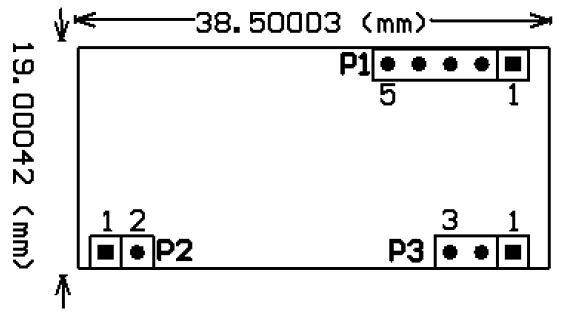
\includegraphics[width=0.4\linewidth]{pre-textuais/figuras/Pinagem_RDM6300}
  \caption{Pinagem do módulo RDM6300}
  \label{Fig:PinagemRDM6300}
  \end{center} \end{figure}

\subsection{Protocolo de Quadros}

O RDM6300 transmite dados através da interface UART utilizando quadros ASCII com estrutura bem definida. A estrutura padrão do quadro é:

\textbf{Formato do Quadro:}
\begin{verbatim}
[HEAD] [DADOS] [CHECKSUM] [TAIL]
\end{verbatim}

Onde:
\begin{itemize}
\item \textbf{HEAD:} 0x02 (início do quadro)
\item \textbf{DADOS:} 10 caracteres hexadecimais ASCII (2 de versão + 8 do ID da tag)
\item \textbf{CHECKSUM:} 2 caracteres hexadecimais ASCII
\item \textbf{TAIL:} 0x03 (fim do quadro)
\end{itemize}

\subsection{Cálculo do Checksum}

O checksum é calculado realizando a operação XOR dos valores numéricos de cada par hexadecimal nos 10 caracteres de dados. Por exemplo, para o número de cartão 62E3086CED:

\begin{itemize}
\item Dados de saída: 36H, 32H, 45H, 33H, 30H, 38H, 36H, 43H, 45H, 44H
\item Cálculo: (62H) XOR (E3H) XOR (08H) XOR (6CH) XOR (EDH) = 08H
\end{itemize}

\subsection{Exemplo Prático de Quadro}

Um exemplo real de saída do módulo:

\textbf{Dados em hexadecimal:}
\begin{verbatim}
02 30 31 30 30 30 37 33 34 45 30 44 32 03
\end{verbatim}

\textbf{Interpretação:}
\begin{itemize}
\item HEAD: 02
\item Dados: 30 31 30 30 30 37 33 34 45 30 (equivale a "0100073E0" em ASCII)
\item Checksum: 44 32 (equivale a "D2" em ASCII)
\item TAIL: 03
\end{itemize}

\textbf{Verificação do checksum:}
(01H) XOR (00H) XOR (07H) XOR (34H) XOR (E0H) = D2H[ç]

\subsection{Considerações de Implementação}

O protocolo facilita a validação local e o descarte de quadros corrompidos através do checksum. Dependendo do cartão ou etiqueta utilizada, o UID efetivo pode ser representado com 8 ou 10 caracteres hexadecimais, sendo necessário que o software acomode ambas as possibilidades \cite{seeed-rfid-125khz}.

Para integração com microcontroladores, um código básico em Arduino seria:

\begin{verbatim}
void setup() {
    Serial.begin(9600);
}

void loop() {
    if(Serial.available()) {
        while(Serial.available()) {
            Serial.write(Serial.read());
        }
    }
}
\end{verbatim}

\section{Controlador DigiProx SA202}
\label{sec:digiprox-sa202}

O DigiProx SA202 é um controlador de acesso dedicado que opera na frequência de 125 kHz, projetado especificamente para controle de entrada e saída de pessoas em pequenos ambientes. Este dispositivo representa uma solução integrada que combina leitor RFID, processamento de autenticação e controle de atuadores em um único equipamento \cite{intelbras-digiprox-sa202}.

\subsection{Especificações Técnicas}

O controlador apresenta as seguintes características técnicas \cite{intelbras-digiprox-sa202}:

\textbf{Especificações Elétricas:}
\begin{itemize}
\item \textbf{Tensão de alimentação:} 12 Vdc
\item \textbf{Potência de operação:} 0,5 W
\item \textbf{Corrente de chaveamento:} 200 mA
\end{itemize}



\textbf{Condições Ambientais:}
\begin{itemize}
\item \textbf{Temperatura de operação:} -10°C a 70°C
\item \textbf{Umidade de operação:} 20\% a 80\%
\end{itemize}

\textbf{Especificações RFID:}
\begin{itemize}
\item \textbf{Frequência de operação:} 125 kHz
\item \textbf{Modulação:} ASK (Amplitude Shift Keying)
\item \textbf{Taxa de transmissão:} 3,906 kbps
\item \textbf{Código de emissão:} 125KA2DCN
\item \textbf{Tipo de antena:} Interna
\end{itemize}

\textbf{Capacidades de Armazenamento:}
\begin{itemize}
\item \textbf{Capacidade máxima de cartões:} 1.000 usuários
\item \textbf{Capacidade máxima de senhas:} 1.000 usuários
\end{itemize}

\textbf{Dimensões Físicas:}
\begin{itemize}
\item \textbf{Dimensões (L × A × P):} 75 × 118 × 21 mm
\item \textbf{Gabinete:} Plástico de alta resistência
\end{itemize}

\subsection{Funcionalidades}

O DigiProx SA202 oferece as seguintes funcionalidades \cite{intelbras-digiprox-sa202}:

\begin{itemize}
\item \textbf{Sinalização sonora:} Feedback auditivo para operações
\item \textbf{Compatibilidade ampla:} Funciona com fechaduras eletroímã, eletromecânicas, leitores e automatizadores de portão
\item \textbf{Métodos de autenticação:} Cartão de proximidade, senha ou acesso combinado
\item \textbf{Controle de usuários:} Gerenciamento de até 1.000 usuários simultâneos
\end{itemize}

\section{Comunicação Serial e Internet das Coisas (IoT)}
\label{sec:comunicacao-iot}

\subsection{Universal Asynchronous Receiver-Transmitter (UART)}

UART é um protocolo de comunicação serial assíncrono amplamente utilizado em sistemas embarcados para transmissão de dados entre dispositivos. Diferente de protocolos síncronos como SPI ou I2C, o UART não requer um sinal de clock compartilhado, tornando-o ideal para comunicações simples entre microcontroladores \cite{makerhero-esp8266}.

Na comunicação UART, os dados são transmitidos bit a bit através de dois fios: TX (transmissão) e RX (recepção). Cada dispositivo possui seu próprio TX conectado ao RX do outro dispositivo, formando uma comunicação full-duplex. A taxa de transmissão (baud rate) deve ser configurada igualmente em ambos os dispositivos para garantir a correta interpretação dos dados.

\subsection{Internet das Coisas (IoT)}

A Internet das Coisas refere-se à interconexão de dispositivos físicos através da internet, permitindo coleta e troca de dados sem intervenção humana direta. No contexto de controle de acesso, IoT possibilita o monitoramento remoto, gestão centralizada e análise de dados em tempo real \cite{embarcados-serial}.

\section{Ponte Microcontrolada e Integração com ESP8266}
\label{sec:ponte-microcontrolada}

A solução proposta adota uma estratégia de separação de responsabilidades entre dois microcontroladores, visando reduzir o acoplamento e facilitar a manutenção e evolução do sistema. Esta abordagem permite que cada componente se especialize em suas funções específicas.

\subsection{Divisão de Responsabilidades}

\textbf{Microcontrolador A (Arduino):}
\begin{itemize}
\item \textbf{Função principal:} Leitura e validação do quadro RFID
\item \textbf{Processamento:} Decodificação do protocolo RDM6300, validação de checksum
\item \textbf{Saída:} Transmissão da TAG em formato texto simples via UART
\item \textbf{Vantagens:} Processamento dedicado, isolamento de falhas, facilidade de teste
\end{itemize}

\textbf{Microcontrolador B (ESP8266):}
\begin{itemize}
\item \textbf{Função principal:} Normalização de dados e comunicação com backend
\item \textbf{Processamento:} Validações finais, formatação JSON, envio HTTPS
\item \textbf{Conectividade:} Interface Wi-Fi, cliente HTTP/HTTPS
\item \textbf{Vantagens:} Evolução independente, conectividade nativa, processamento de rede
\end{itemize}

\subsection{Benefícios da Arquitetura}

Esta separação oferece vantagens significativas:

\begin{itemize}
\item \textbf{Redução de acoplamento:} Cada módulo tem responsabilidades bem definidas
\item \textbf{Facilidade de testes:} Testes em bancada podem ser realizados independentemente
\item \textbf{Evolução independente:} O envio à nuvem pode evoluir sem afetar a leitura RFID
\item \textbf{Isolamento de falhas:} Problemas de conectividade não afetam a leitura local
\item \textbf{Manutenibilidade:} Código mais modular e fácil de manter
\end{itemize}

\section{Plataforma Wi-Fi para IoT: ESP8266}
\label{sec:esp8266-wifi}

O ESP8266 é um System-on-Chip (SoC) desenvolvido pela Espressif Systems que integra um processador de 32 bits com conectividade Wi-Fi 802.11 b/g/n. Lançado em 2014, rapidamente se tornou uma das plataformas mais populares para projetos IoT devido ao seu baixo custo e facilidade de programação \cite{makerhero-esp8266,embarcados-serial}.

\subsection{Especificações Técnicas}

O ESP8266 apresenta características que o tornam ideal para aplicações IoT \cite{espressif-esp8266}:

\begin{itemize}
\item \textbf{Processador:} Tensilica L106 de 32 bits operando a 80/160 MHz
\item \textbf{Memória:} 64 KB de RAM de instruções e 96 KB de RAM de dados
\item \textbf{Conectividade:} Wi-Fi 802.11 b/g/n com WPA/WPA2
\item \textbf{Protocolos:} Pilha TCP/IP completa, suporte a IPv4
\item \textbf{Programação:} Compatível com Arduino IDE, MicroPython e SDK nativo
\item \textbf{Interfaces:} UART, SPI, I2C, PWM e GPIO
\end{itemize}

\subsection{Implementação de Servidor HTTP Local}

O ESP8266 pode hospedar um servidor HTTP local para testes e configuração:

\begin{verbatim}
// Exemplo de endpoint para testes
GET /setTag?code=1A2B3C4D
POST /api/access
{
  "tag": "1A2B3C4D",
  "timestamp": 1712345678,
  "device": "ESP8266-ABCD"
}
\end{verbatim}

\subsection{Limitações e Considerações}

\textbf{Restrições de Hardware:}
\begin{itemize}
\item \textbf{RAM limitada:} Requer gerenciamento cuidadoso de memória
\item \textbf{Flash limitado:} Código deve ser otimizado
\item \textbf{Processamento:} Single-core, requer programação não-bloqueante
\end{itemize}

\textbf{Confiabilidade de Rede:}
\begin{itemize}
\item \textbf{Reconexão automática:} Rotinas para reconectar Wi-Fi
\item \textbf{Timeouts:} Configuração adequada de timeouts HTTP
\item \textbf{Fila offline:} Sistema store-and-forward para garantir entrega
\item \textbf{Retry logic:} Tentativas com backoff exponencial
\end{itemize}

\section{Serviços Web, REST e JSON}
\label{sec:rest-json}

A arquitetura REST (Representational State Transfer) é um estilo arquitetural para sistemas distribuídos proposto por Roy Fielding em 2000. REST modela recursos como URLs e utiliza métodos HTTP padrão para manipulá-los, sendo amplamente adotada em sistemas IoT devido à sua simplicidade e interoperabilidade \cite{restful-api-tutorial}. O formato JSON (JavaScript Object Notation) tornou-se o padrão de facto para troca de dados em APIs REST por sua leveza e facilidade de leitura \cite{mdn-json}.

\subsection{Princípios REST e Métodos HTTP}

Os métodos HTTP definem as operações que podem ser realizadas sobre recursos \cite{mdn-http-methods}:

\begin{itemize}
\item \textbf{GET:} Recuperação de recursos sem efeitos colaterais (idempotente e seguro)
\item \textbf{POST:} Criação de novos recursos ou envio de dados para processamento (não idempotente)
\item \textbf{PUT:} Atualização completa de recursos existentes (idempotente)
\item \textbf{DELETE:} Remoção de recursos do servidor (idempotente)
\end{itemize}

A idempotência é uma propriedade importante que garante que múltiplas chamadas idênticas produzem o mesmo resultado, fundamental para a confiabilidade em redes instáveis \cite{restful-api-tutorial}.

\textbf{Representação JSON:}
\begin{verbatim}
{
  "tag": "1A2B3C4D",
  "timestamp": 1712345678,
  "device": "ESP8266-ABCD",
  "reader": "RDM6300",
  "door": "entrance_01"\subsubsection*{Subsubseções}
  %\label{Sec:subsubsecoes}
  
\end{verbatim}

\subsection{Vantagens para Dispositivos Embarcados}

\begin{itemize}
\item \textbf{Simplicidade:} Protocolo bem definido e amplamente conhecido
\item \textbf{Interoperabilidade:} Compatível com qualquer cliente HTTP
\item \textbf{Debug facilitado:} Ferramentas padrão (curl, Postman, navegadores)
\item \textbf{Escalabilidade:} Stateless por natureza
\end{itemize}

\section{Firebase Realtime Database via REST}
\label{sec:firebase-rtdb}

O Firebase Realtime Database (RTDB) oferece uma API REST completa que permite operações CRUD através de requisições HTTP padrão \cite{firebase-rtdb}.

\subsection{Estrutura da API REST}

\textbf{Endpoint padrão:}
\begin{verbatim}
POST https://<project-id>-default-rtdb.firebaseio.com/<path>.json?auth=<TOKEN>
\end{verbatim}

\textbf{Exemplo de requisição:}
\begin{verbatim}
POST https://meu-projeto.firebaseio.com/access_logs.json?auth=<TOKEN>
Content-Type: application/json

{
  "tag": "1A2B3C4D",
  "timestamp": 1712345678,
  "device": "ESP8266-ABCD"
}
\end{verbatim}

\subsection{Autenticação e Segurança}

\begin{itemize}
\item \textbf{Token de autenticação:} Parâmetro auth na URL
\item \textbf{Regras de segurança:} Restrição de leitura/escrita por dispositivo/usuário
\item \textbf{HTTPS obrigatório:} Comunicação criptografada
\item \textbf{Validação de certificado:} Verificação da cadeia de confiança
\end{itemize}

\section{HTTPS/TLS em Embarcados}
\label{sec:https-tls}

A comunicação segura é essencial para sistemas de controle de acesso, exigindo implementação adequada de TLS no ESP8266 \cite{mdn-https,esp8266-bearssl}.

\subsection{Implementação BearSSL}

O ESP8266 utiliza BearSSL como implementação padrão de TLS, oferecendo diferentes abordagens de validação:

\textbf{Opções de Validação:}
\begin{itemize}
\item \textbf{CA Root:} Validação através da cadeia de confiança completa
\item \textbf{Certificate Pinning:} Fixação da impressão digital do certificado
\item \textbf{Modo inseguro:} Apenas para desenvolvimento (setInsecure())
\end{itemize}

\subsection{Boas Práticas de Segurança}

\begin{itemize}
\item \textbf{Evitar modo inseguro:} Nunca usar setInsecure() em produção
\item \textbf{Timeouts adequados:} Configurar timeouts para conexões TLS
\item \textbf{Retry com backoff:} Tentativas exponenciais em caso de falha
\item \textbf{Validação de certificado:} Sempre validar a cadeia de confiança
\end{itemize}

\section{Sincronização Temporal (NTP)}
\label{sec:ntp-sync}

Para registros auditáveis e análises temporais confiáveis, a sincronização temporal é fundamental em sistemas de controle de acesso \cite{nic-br-ntp,observatorio-nacional}.

\subsection{Estratégias de Sincronização}

Para garantir a precisão temporal no sistema, implementei diversas estratégias de sincronização. A primeira delas é a sincronização obrigatória durante o boot do dispositivo, garantindo que o sistema sempre inicie com o horário correto. Além disso, configurei uma ressincronização periódica a cada 24 horas para manter a precisão ao longo do tempo. Para compensar possíveis desvios do relógio interno do ESP8266, implementei um mecanismo de correção de deriva que ajusta gradualmente pequenas diferenças detectadas. Como medida de contingência, caso ocorra alguma falha na sincronização NTP, o sistema utiliza timestamps relativos baseados no tempo de funcionamento do dispositivo, garantindo que os registros mantenham sua ordem cronológica mesmo sem acesso ao servidor de tempo.

\subsection{Modelagem de Dados}

\textbf{Esquema mínimo recomendado:}
\begin{verbatim}
{
  "tag": "1A2B3C4D",
  "timestamp": 1712345678,
  "device": "ESP8266-ABCD",
  "reader": "RDM6300",
  "door": "entrance_01"
}
\end{verbatim}

\subsection{Práticas de Confiabilidade}

Para garantir a confiabilidade do sistema, implementei várias práticas essenciais. A normalização estrita dos dados através da validação do formato hexadecimal dos cartões RFID garante que apenas leituras válidas sejam processadas. A implementação de idempotência previne o registro duplicado de eventos, mesmo em casos de reenvio de dados. Quando o dispositivo está offline, utilizo uma estratégia de store-and-forward, mantendo os eventos em uma fila local até que a conexão seja restabelecida. Em casos de falha de comunicação, aplico um algoritmo de backoff exponencial para os retries, evitando sobrecarga do servidor. Cada dispositivo possui um identificador único (UID) que permite rastrear a origem de cada evento no sistema. Por fim, todos os logs são estruturados de forma padronizada, facilitando tanto o troubleshooting quanto a auditoria posterior dos eventos.

\section{Síntese e Implicações}
\label{sec:sintese}

A fundamentação teórica apresentada estabelece os pilares técnicos necessários para implementação de um sistema completo de controle de acesso baseado em RFID com conectividade IoT. A literatura e documentação levantadas fundamentam: (a) a leitura confiável de RFID LF (125 kHz) e seus efeitos práticos \cite{vieira-rfid-2007,avery-dennison-rfid}; (b) o parse de quadros ASCII do RDM6300 com checksum XOR para integridade \cite{seeed-rfid-125khz}; (c) a arquitetura de ponte UART com validação no Arduino e publicação REST no ESP8266 \cite{embarcados-serial,makerhero-esp8266}; (d) o envio HTTPS com práticas de segurança mínimas \cite{mdn-https,firebase-rtdb}; e (e) elementos de formatação acadêmica e reprodutibilidade exigidos em TCC \cite{abnt-2018,abnt-2023,abnt-2024}.

\subsection{Componentes Integrados}

A solução desenvolvida neste trabalho integra múltiplos componentes tecnológicos de forma harmoniosa. A leitura RFID é realizada através do protocolo RDM6300 com validação de integridade dos dados, garantindo confiabilidade nas leituras. A arquitetura distribuída separa as responsabilidades entre os microcontroladores Arduino e ESP8266, permitindo que cada um execute as tarefas para as quais é mais adequado. A conectividade com a nuvem é estabelecida de forma segura através de HTTPS/TLS com validação adequada dos certificados CA pré-configurados para validação de servidores populares como Google, Firebase e AWS estão disponíveis na biblioteca BearSSL do ESP8266, simplificando a implementação de conexões seguras. A sincronização temporal via NTP garante timestamps auditáveis para todos os eventos registrados. Além disso, implementei práticas robustas de confiabilidade com tratamento adequado de falhas e mecanismos de recuperação automática.

\subsection{Reprodutibilidade e Padrões}

Para garantir a reprodutibilidade do projeto, todos os componentes foram especificados seguindo protocolos padronizados como UART para comunicação serial, HTTP/HTTPS para comunicação web, JSON para estruturação de dados e NTP para sincronização temporal. A implementação baseia-se exclusivamente em documentação oficial dos fabricantes e organizações de padrões, seguindo as práticas estabelecidas pela indústria para desenvolvimento de soluções IoT. Todo o código desenvolvido está documentado e disponível como referência para implementações futuras.

Esses pilares tornam o trabalho auto-contido e reproduzível, pois todos os blocos (protocolo, UART, REST/HTTPS, estrutura do dado) estão especificados e suportados por referências, fornecendo base sólida para a implementação prática do sistema de controle de acesso.

